\subsection{Server}\label{subsec: Server}
Als Server für die Openhab Software wird ein Raspberrypi der 4. Generation mit 2 GB RAM eingesetzt, die Installation und Inbetriebnahme wird im Benutzerhandbuch beschrieben. In Openhab wird ebenfalls ein eigener MQTT-Broker eingebunden. Damit diese Broker von jedem Gerät im Lokalen Netzwerk erreicht werden kann, wird dem Server eine Statische IP Adresse vergeben.\\
\\
Um den Sprachassistent einzubinden ist ein weiterer Server mit der Home Assistant Software in das System Integriert worden. Dieser Server wurde auf ein Rasperrypi 4. Generation 2 GB RAM installiert. Der Grund warum nicht beide Server auf dem selben Raspberrypi installiert wurden, ist einerseits, das System ist physikalisch Modular aufgebaut der Sprach Assistent Teil kann als separates Thing (Gerät) betrachtet werden. Andererseits, wenn sich beide Server auf dem Selben Gerät befinden wäre die MQTT-Kommunikation sinnlos.  



\begin{figure}[H]
	\centering
	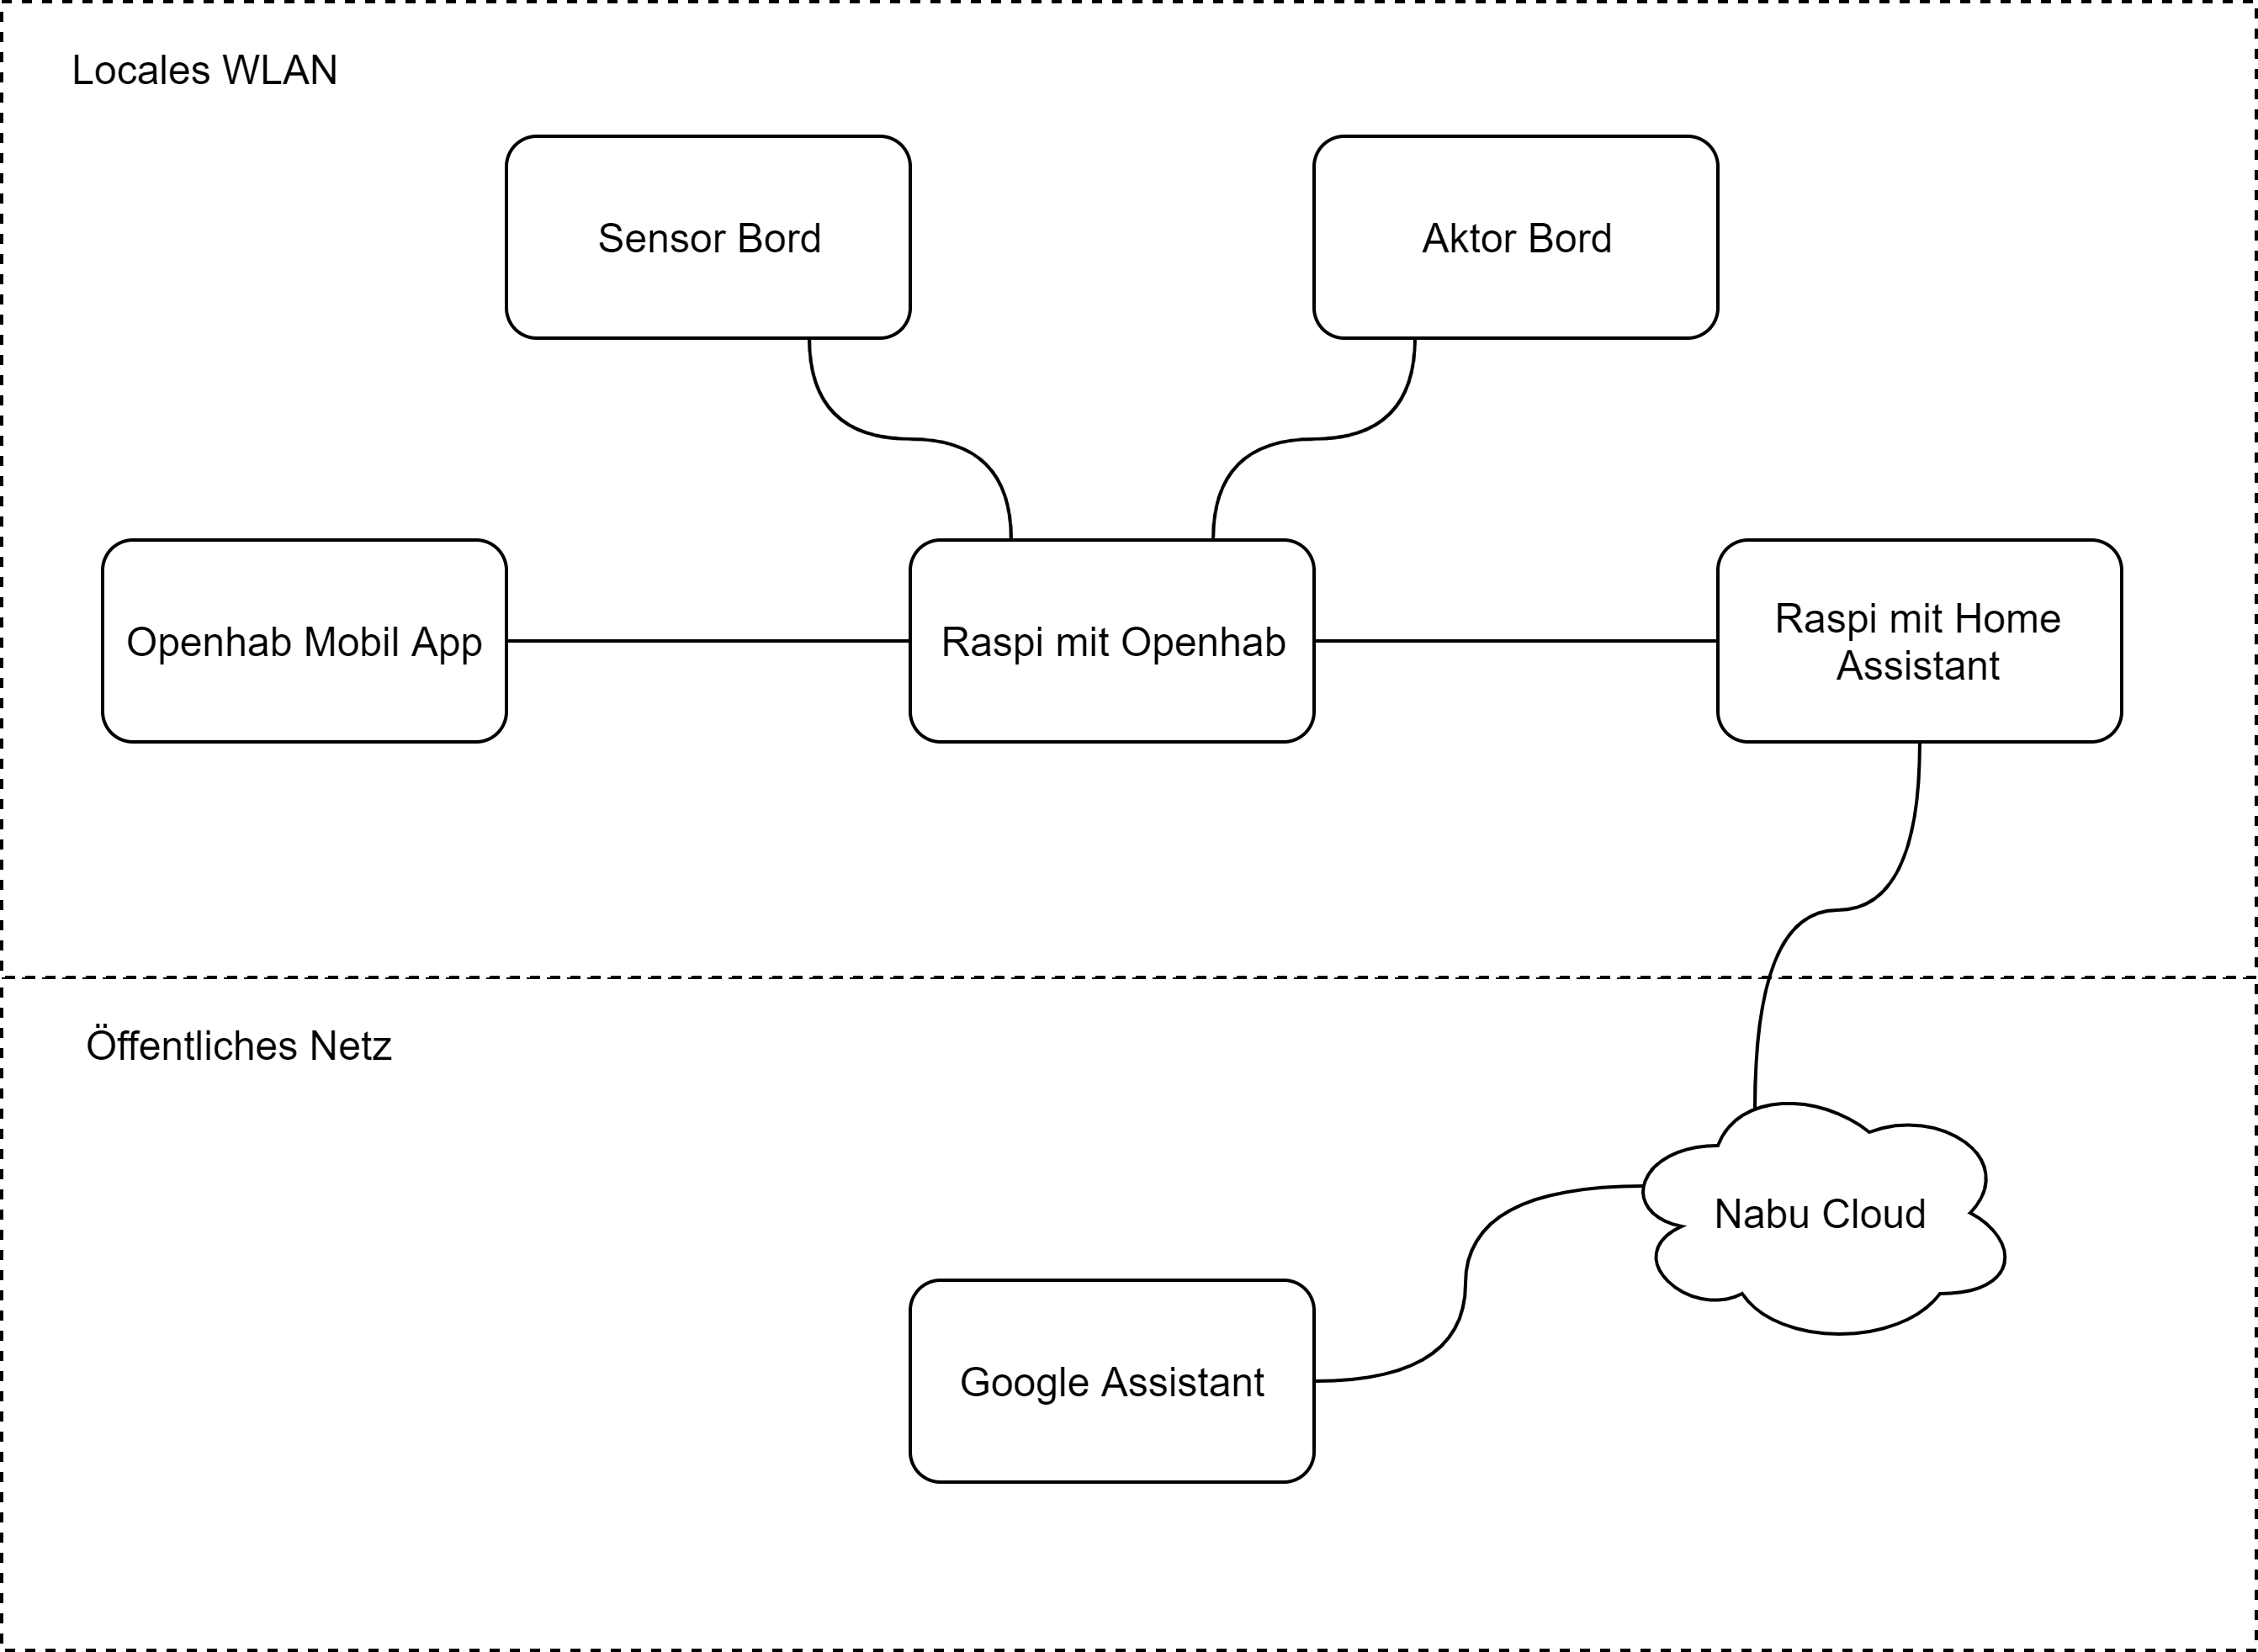
\includegraphics[width=\textwidth]{graphics/Systemubersicht.png}
	\caption{Systemübersicht}
	\label{pic: Systemübersicht}
\end{figure}   

In der Abbildung \ref{pic: Systemübersicht} kann erkannt werden, dass sich beide Server im selben Lokalen Netzwerk befinden. Die Kommunikation zwischen den beiden Server findet über MQTT statt, es besteht die Möglichkeit den Openhab-Server zu umgehen und eine direkte Kommunikation vom Home Assistant zu dem Sensor- oder zum Aktorbord zu realisieren. In diesem Fall müssen aber die Regeln bei welchem Aktion, welche Schalthandlung ausgelösst wird, in den entsprechenden Mikrocontroller Programmiert werden.

